\documentclass[11pt]{article}
\usepackage[a4paper, left=2cm, right=2cm]{geometry}

\usepackage[utf8]{inputenc}
\usepackage[english]{babel}
\usepackage[T1]{fontenc}
\usepackage{amsmath}
\usepackage{amsfonts}
\usepackage{amssymb}
\usepackage{tablefootnote}
\usepackage{graphicx}
\usepackage{longtable}

\usepackage{url}

\usepackage{siunitx}
\sisetup{
    round-mode=places,
    round-precision = 3,
}

% center fixed width:
\newcolumntype{C}[1]{>{\centering\arraybackslash}p{#1}}
\newcolumntype{L}[1]{>{\raggedright\arraybackslash}p{#1}}

\bibliographystyle{ieeetr}  
\usepackage[backend=biber]{biblatex}
\addbibresource{Sources.bib}   
%\title{Customizing Bibliography: \texttt{biblatex} package}

\usepackage{fancyhdr}
\pagestyle{fancy}
\usepackage{enumitem}
\author{Hanna Gloyna}
\title{Sarcopenia Dataset\\
		\large Writting Report: Statistical Analysis}
\setlength{\headheight}{40pt}
\date{}
\pagenumbering{Roman}
\lhead{Sarcopenia Dataset}

\begin{document}
\twocolumn
\maketitle
\thispagestyle{fancy}

\section{Statistical Analysis}
The used data set contained initially 250 entries, where each entry represents a patient, with 84 features. After removing ID, 17 entries were deleted as they were duplicates. Furthermore 8 misses in \emph{Marcha} (engl. walking speed) were imputed with the mean. The encoding of the categorical data was changed, so that afterwards $0$ did always correspond to either \emph{Not answered}, \emph{Not required} or \emph{Regular value}. To obtain comparable values for variance of each feature a min-max-normalisation was applied, given by Equation \ref{eq:minmax}.

\begin{equation}\label{eq:minmax}
\hat{x} = \frac{x-min(x)}{max(x)-min(x)}
\end{equation}

Where $x$ corresponds to the original value of a feature, $min(x)$ the minimal values of this feature and $max(x)$ to the maximal value, respectively. Afterwards all features are within $\left[0,1\right]$.

In accordance with specialists every representation of MMSE, Barthel, Norton, Lawton, and MNA, except the binary, was removed to reduce the dimensionality of the datset. Additionally MM was dropped, because of its high correlation to IMM.

We dropped further features with too low variance or entropy, i.e. 90\% of the values were the same. Additionally 7 features were deleted, because they contained a lot of misses or were included in another feature. Afterwards again all duplicates were dropped.

The remaining 231 entries included 42 serve and 189 mild sarcopenia cases. The study consists of 166 women and 65 men between 60 to 97 years old and a median age of 79. By definition a serve sarcopenia cases is a decrease of IMM, grip strength and walking pace. If only a decrease of IMM and grip strength or walking speed is detected, it is classified as a mild case. With this definition 24 of 42 serve cases could be selected, whereas 18 serve cases did not match the definition and 7 cases would be serve by definition, but were not marked as such.

% table with p value and f1 result
\begin{table}[t]
\centering
\begin{tabular}{|c|S S|}
\hline
Feature & $\text{p}$		& $\text{f1}$ \\ \hline
TNCM	& 0.000403	& 14.971373\\
Demencia& 0.000654 	& 15.254129\\
FuerzaPrension &  0.005826    &   8.956896\\
Pantorrilla &   0.097496       &  40.598309\\
IMM & 0.135147   &  24.095192\\
LawtonAR &    0.171091   &   3.151468\\
Dolor &     0.173250  &   2.866794\\
Congiciòn &     0.173992    &   4.143239\\
Charlson &    0.177932  &   2.372304\\
CorreccionVisual &  0.195190  &   9.427020\\
\hline
%7   Ocupacion  	 0.214646      8.094724
%39  NortonAlto      0.386392      7.721943
%1   Edad		     0.557026      4.422385
\end{tabular}
\caption{Features and their corresponding p-value and f1-value to \emph{sarcopenia} }
\label{table:chi2_anova}
\end{table}

The features with the highest Spearman correlation coefficient $r_s$ are listed in Table \ref{table:corr}. The used threshold for a high correlation was $|r_s| > 0,7$ as suggested by Akoglu in \cite{akoglu_users_2018}. In each row of Table \ref{table:corr} either feature 1 or feature 2 could be removed.

% table with high correlation coefficients
\begin{table}[t]
\centering
\begin{tabular}{|c c|S|}
\hline
Feature 1 & Feature 2 & $r_s$ \\ \hline
OA&Visiòn&-0.7694806696505007\\
MED8&MED7& 0.7587853686054055\\
Drogas&Visiòn&-0.7028060168312469\\ \hline
\end{tabular}
\caption{Features with high correlation coefficient}
\label{table:corr}
\end{table}

\begin{table}[b]
\centering
\begin{tabular}{|L{0.6\columnwidth}|C{0.25\columnwidth}|}
\hline
Features & Method \\ \hline
CorreccionVisual, TNCM, LawtonAR, Charlson, \textbf{IMM}, FuerzaPrension, \textbf{Pantorrilla}, Demencia, Congiciòn, Dolor & $\chi_2$ \\ \hline
Edad, Ocupacion, CorreccionVisual, TNCM, NortonAlto, \textbf{IMM}, FuerzaPrension, \textbf{Pantorrilla}, Demencia, Congiciòn & f1 score\\ \hline
Edad, Ocupacion, MED1, MED2, MED4, MED5, \textbf{IMM}, AnguloF, \textbf{Pantorrilla}, Marcha & RFE with RF \\ \hline
CorreccionVisual, TNCM, IMM, FuerzaPrension, Pantorrilla, Demencia, Congiciòn & Intersection of $\chi_2$ and f1 score\\ \hline
\end{tabular}
\caption{Most important features according to \emph{Method}}
\label{table:feature_selection}
\end{table}

\begin{figure*}[t]
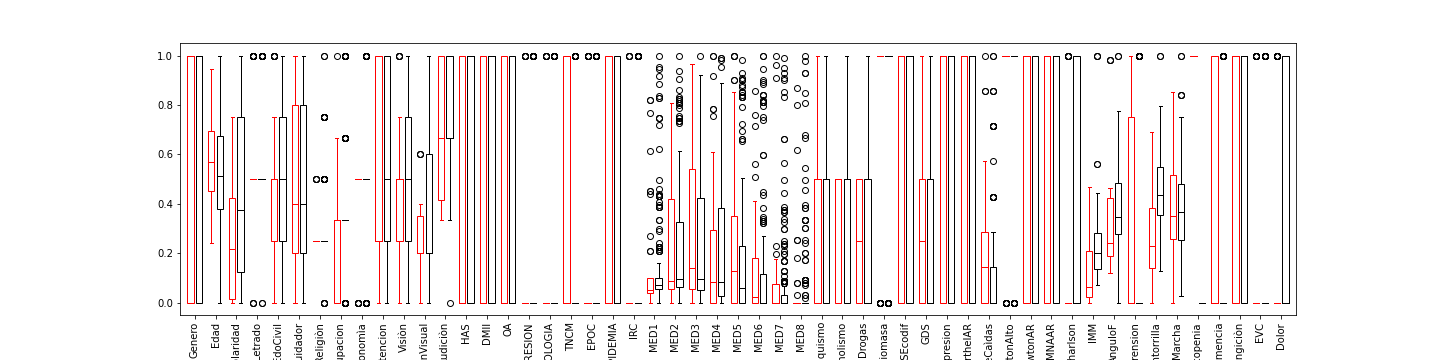
\includegraphics[width=\linewidth]{boxplot_serve_mild.png}
\caption{Boxplot of all remaining features, black boxes are created from all mild cases and red from all serve, respectively}
\label{fig:boxplots}
\end{figure*}

The results of a $\chi_2$ and \emph{ANOVA} analysis are displayed in Table \ref{table:chi2_anova}. The 10 features with the lowest p-value from $\chi_2$ analysis are almost the same as the ones with the highest f1 score. Only Ocupacion, NortonAlto and Edad (engl. age) achieved a higher f1 score, but a had also a higher p-value.


Figure \ref{fig:boxplots} displays the plotted boxes of all remaining 53 features, where black boxes are generated from the subset of mild cases and red boxes from serve cases, respectively. Features with a difference at their mean and inter quartile range are especially interesting and very likely to be important for decision making. As can be seen features such as TNCM, Charlson, IMM, FuerzaPrension, Demencia and Dolor vary a lot for serve and mild cases. This also supports the calculated values and assignment of importance from the calculation of the p- and f1-value.

\section{Hyperparameter Tuning}
\begin{figure*}[t]
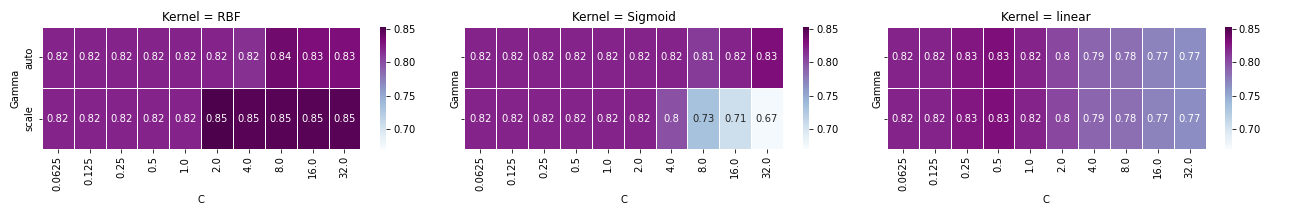
\includegraphics[width=\linewidth]{heatmap_svc_hyperparameter.png}
\caption{Results of hyperparameter tuning for SVM}
\label{fig:hyper_svc}
\end{figure*}

A \emph{Support Vector Machine} (hereinafter: SVM) was used to predict the severity of sarcopenia. A cross validated grid search was applied to get an impression which setting of parameters might be a good fit. Fig. \ref{fig:hyper_svc} displays the results, where \emph{C}, $\gamma$ and 3 different kernels were considered. In every setting the \emph{Radial Basis Function} (rbf) did perform at least as good as the two other kernel. Furthermore it can be clearly seen that $C=2$ and $\gamma=scale$ are the best setting with the rbf kernel.

\begin{figure*}[t]
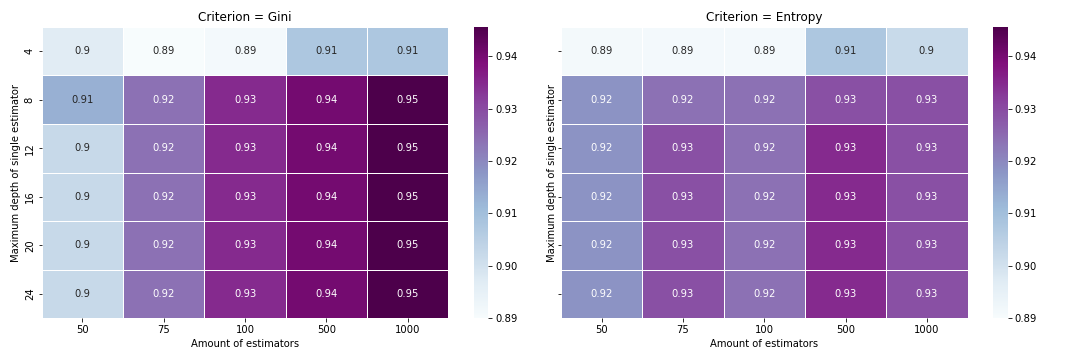
\includegraphics[width=\linewidth]{heatmap_rf_hyperparameter.png}
\caption{Results of hyperparameter tuning for RF}
\label{fig:hyper_rf}
\end{figure*}

Beside the SVM also a \emph{Random Forest} (hereinafter: RF) was trained. Again a cross validated grid search was used. For tuning the depth $d$ of the trees in a set $S$, amount of trees $|S|$ as well as the splitting criteria were considered. As can be seen in Fig. \ref{fig:hyper_rf} there is no huge difference between the splitting criteria and a RF performed best with its parameters as follows: $|S|= 75, criteria = gini, d=20$.


\section{Feature Selection}
By calculating the p-value and f1 score between each feature and sarcopenia we can get an idea for feature selection. A low p-value indicates that the two features are independent and therefore provide information about each other regarding predictions by statistical models. Table \ref{table:feature_selection} displays the 10 most important features for different methods such as $\chi_2$, ANOVA and recursive feature elimination (hereinafter: RFE) with a RF as an estimator. Furthermore it lists the intersection of the methods, which gives an idea what attributes are most important for generalisation. Features which appear in every ranking of the 10 most important feature are marked bold.



\printbibliography[heading=bibintoc, title={References}]
\end{document}
